% =====================================================================================
%  Retail25 — Software Stack Documentation
%
%  Generated from repository evidence on branch `main`, worktree
%  .claude/worktrees/phase-3-4-completion-0addae, at commit e7f91ad.
%
%  Every technology and version in this document was read out of a file in the
%  repository. Where a fact could not be established from the repository it is
%  labelled Not Verified rather than guessed.
%
%  Build:  latexmk -pdf software_stack_documentation.tex
%     or:  pdflatex software_stack_documentation.tex   (run three times)
% =====================================================================================
\documentclass[11pt,a4paper]{report}

\usepackage[T1]{fontenc}
\usepackage[utf8]{inputenc}
\usepackage{lmodern}
\usepackage[a4paper,margin=2.4cm,headheight=15pt]{geometry}
\usepackage{graphicx}
\usepackage{xcolor}
\usepackage{booktabs}
\usepackage{longtable}
\usepackage{tabularx}
\usepackage{array}
\usepackage{float}
\usepackage{enumitem}
\usepackage{fancyhdr}
\usepackage{amsmath}
\usepackage{tikz}
\usepackage{pdflscape}
\usepackage[hidelinks,bookmarksnumbered]{hyperref}
\usepackage{bookmark}

\usetikzlibrary{shapes.geometric,arrows.meta,positioning,fit,backgrounds,calc}

% ---- line breaking ------------------------------------------------------------------
% An identifier like AllowAuthorizationCodeFlow() has no separator to break at, and TeX
% will not hyphenate a word containing parentheses. Without an escape valve such a word
% simply runs past the margin. \emergencystretch buys a final pass with looser word
% spacing instead, which is the lesser of the two uglinesses.
\setlength{\emergencystretch}{3em}
\tolerance=2000
\hyphenpenalty=100

% ---- palette ------------------------------------------------------------------------
\definecolor{r25ink}{HTML}{1A1F2B}
\definecolor{r25muted}{HTML}{5B6478}
\definecolor{r25rule}{HTML}{C8CEDA}
\definecolor{r25front}{HTML}{3B6FD4}
\definecolor{r25back}{HTML}{2E7D64}
\definecolor{r25data}{HTML}{8A5A1E}
\definecolor{r25edge}{HTML}{7A3E9D}
\definecolor{r25infra}{HTML}{4A5568}
\definecolor{r25frontbg}{HTML}{E8EFFC}
\definecolor{r25backbg}{HTML}{E4F2EC}
\definecolor{r25databg}{HTML}{F7EEDD}
\definecolor{r25edgebg}{HTML}{F1E8F8}
\definecolor{r25infrabg}{HTML}{EDEFF3}

% ---- headers ------------------------------------------------------------------------
\pagestyle{fancy}
\fancyhf{}
\fancyhead[L]{\small\color{r25muted}Retail25 — Software Stack Documentation}
\fancyhead[R]{\small\color{r25muted}\thepage}
\renewcommand{\headrulewidth}{0.4pt}
\renewcommand{\headrule}{\hbox to\headwidth{\color{r25rule}\leaders\hrule height \headrulewidth\hfill}}

% ---- helpers ------------------------------------------------------------------------
% File paths and identifiers. Underscores are escaped at the call site as \us.
%
% A path is one unbreakable word to TeX: there is no letter pair in
% `app/api/proxy/[...]/route.ts' that it may hyphenate, so a 2.8cm table column cannot
% hold it and the text simply runs off the page edge. Seventy-six boxes overflowed, one
% of them by 7cm, before these existed.
%
% The separators are made break opportunities instead. The catcodes have to change
% before the argument is tokenised, which is why each of these is two macros: the first
% opens a group and switches the catcodes, the second then reads the argument.
\newcommand{\rslash}{\char47}
\newcommand{\rdot}{\char46}
\newcommand{\rdash}{\char45}
\newcommand{\rat}{\char64}

\begingroup
  \catcode`\/=\active
  \catcode`\.=\active
  \catcode`\-=\active
  \catcode`\@=\active
  % \allowbreak, not \- : a path must never acquire a hyphen it did not have.
  \gdef\rbreaks{%
    \def/{\rslash\allowbreak}%
    \def.{\rdot\allowbreak}%
    \def-{\rdash\allowbreak}%
    \def@{\rat\allowbreak}%
  }%
\endgroup

\newcommand{\ractive}{%
  \catcode`\/=\active \catcode`\.=\active \catcode`\-=\active \catcode`\@=\active
  \rbreaks}

\newcommand{\pathx}{\begingroup\ractive\rpathfin}
\newcommand{\rpathfin}[1]{{\small\ttfamily #1}\endgroup}

\newcommand{\code}{\begingroup\ractive\rcodefin}
\newcommand{\rcodefin}[1]{{\small\ttfamily #1}\endgroup}

% Package names, which break at @ and - as well as /.
\newcommand{\pkg}{\begingroup\ractive\rpkgfin}
\newcommand{\rpkgfin}[1]{{\ttfamily #1}\endgroup}

\newcommand{\us}{\char`_}

% Verification labels
\newcommand{\vok}{\textcolor{r25back}{\textbf{Verified}}}
\newcommand{\vder}{\textcolor{r25data}{\textbf{Derived}}}
\newcommand{\vrec}{\textcolor{r25front}{\textbf{Recommended}}}
\newcommand{\vno}{\textcolor{r25muted}{\textbf{Not Verified}}}
\newcommand{\vna}{\textcolor{r25muted}{\textbf{N/A}}}

\newcolumntype{L}[1]{>{\raggedright\arraybackslash}p{#1}}

% ---- tikz styles --------------------------------------------------------------------
\tikzset{
  box/.style   = {rectangle, rounded corners=2pt, draw, thick, align=center,
                  minimum height=9mm, inner sep=4pt, font=\scriptsize},
  front/.style = {box, draw=r25front, fill=r25frontbg},
  back/.style  = {box, draw=r25back,  fill=r25backbg},
  data/.style  = {cylinder, shape border rotate=90, aspect=0.25, draw, thick,
                  draw=r25data, fill=r25databg, align=center, font=\scriptsize,
                  minimum height=11mm, inner sep=3pt},
  edge/.style  = {box, draw=r25edge,  fill=r25edgebg},
  infra/.style = {box, draw=r25infra, fill=r25infrabg},
  dec/.style   = {diamond, draw, thick, draw=r25infra, fill=r25infrabg, align=center,
                  font=\scriptsize, aspect=1.6, inner sep=1pt},
  % Named `stage`, not `step`: /tikz/step is a built-in key that takes a value, and
  % redefining it makes pgfkeys reject every node that uses it.
  stage/.style  = {box, draw=r25infra, fill=white},
  flow/.style  = {-{Stealth[length=2mm]}, thick, draw=r25ink},
  flowdash/.style = {-{Stealth[length=2mm]}, thick, dashed, draw=r25muted},
  lbl/.style   = {font=\tiny, fill=white, inner sep=1pt},
}

% =====================================================================================
\begin{document}

% ---- cover --------------------------------------------------------------------------
\begin{titlepage}
\centering
\vspace*{2.2cm}

{\Huge\bfseries\color{r25ink} Retail25\par}
\vspace{4mm}
{\Large\color{r25muted} Software Stack Documentation\par}

\vspace{10mm}
{\color{r25rule}\rule{0.72\textwidth}{1pt}}
\vspace{8mm}

\begin{minipage}{0.80\textwidth}
\centering\color{r25ink}
A self-hosted, web-based Point of Sale, Inventory and Accounts-Receivable
platform, rebuilt from \emph{Retail Plus for Windows 2.5}
(True North Computer Services, 2008), with bulk RFID reading added.
\end{minipage}

\vspace{12mm}

\begin{tabular}{@{}r@{\hspace{6mm}}l@{}}
\textbf{Document} & Software Stack Documentation \\[2pt]
\textbf{Product version} & 0.1.0 \quad{\small(\pathx{backend/Directory.Build.props})} \\[2pt]
\textbf{Repository branch} & \code{main} \\[2pt]
\textbf{Commit} & \code{e7f91ad} \\[2pt]
\textbf{Generated} & 9 October 2026 \\[2pt]
\textbf{Purpose} & Technology inventory, architecture and deployment reference \\
\end{tabular}

\vspace{12mm}

\begin{minipage}{0.86\textwidth}
\small\color{r25ink}
\textbf{Stack at a glance.}
C\# on .NET~10 with Clean Architecture and CQRS (MediatR);
SQL~Server via Entity Framework Core~10;
ASP.NET~Core Web API with SignalR for realtime;
ASP.NET~Core Identity with OpenIddict and JWT bearer schemes;
Next.js~14 (App Router) with React~18, TypeScript and Tailwind~CSS as a
backend-for-frontend; and a Windows-service terminal agent that drives RFID
readers and till peripherals.
\end{minipage}

\vspace{14mm}
{\color{r25rule}\rule{0.72\textwidth}{0.6pt}}
\vspace{4mm}

{\footnotesize\color{r25muted}
Every technology, version and component in this document was read from a file in the
repository. Items that could not be established from the repository are labelled
\emph{Not Verified} rather than inferred.\par}

\vfill
\end{titlepage}

% ---- front matter -------------------------------------------------------------------
\pagenumbering{roman}
\tableofcontents
\clearpage
\listoffigures
\clearpage
\listoftables
\clearpage
\pagenumbering{arabic}
\setcounter{page}{1}

% =====================================================================================
\chapter{Executive Summary}
\label{ch:exec}

Retail25 replaces a 2008 Windows desktop application — \emph{Retail Plus for Windows~2.5} —
with a self-hosted web system covering point of sale, inventory, and accounts receivable.
The legacy system stored data in DBF files on mapped network drives; Retail25 replaces that
with SQL~Server, an ASP.NET~Core API and a Next.js front end, and adds bulk RFID reading that
the original did not have.

\section{What the system is made of}

Five runnable pieces, each verified in the repository:

\begin{itemize}[leftmargin=*,itemsep=3pt]
  \item \textbf{A Web API} (\pathx{backend/src/Retail25.Api}) — ASP.NET~Core controllers under
        \code{api/v1/\ldots}, four SignalR hubs, health endpoints and background jobs.
  \item \textbf{A domain and application core} (\pathx{Retail25.Domain},
        \pathx{Retail25.Application}) — entities, the pricing engine, and CQRS handlers
        dispatched by MediatR.
  \item \textbf{An infrastructure layer} (\pathx{Retail25.Infrastructure}) — EF~Core against
        SQL~Server, ASP.NET~Core Identity, OpenIddict, caching and realtime notifiers.
  \item \textbf{A web front end} (\pathx{frontend}) — Next.js~14 App Router. It is not only a UI:
        its route handlers act as a \emph{backend for frontend}, holding the session cookie and
        proxying to the API so no token ever reaches the browser.
  \item \textbf{A terminal agent} (\pathx{Retail25.TerminalAgent}) — a Windows service installed
        on a till that drives RFID readers, scales, cash drawers and pole displays, and connects
        \emph{outbound} to the server over SignalR.
\end{itemize}

\section{How data is stored and moved}

Persistence is SQL~Server through EF~Core~10 with snake-case naming; the
\code{ApplicationDbContext} exposes 89 entity sets across 12 migrations. Cart state, tag
debouncing and idempotency records are held through a cache provider that defaults to
SQL~Server, with Redis as an explicit opt-in. Browser traffic is HTTPS to the Next.js
server, which calls the API server-to-server; live updates reach the browser over SignalR
WebSockets, authenticated by a single-use ticket rather than a token.

\section{How it is built and shipped}

Continuous integration (\pathx{.github/workflows/ci.yml}) runs four jobs — backend tests,
frontend checks, end-to-end browser tests and container image builds. A separate pipeline
(\pathx{.github/workflows/deploy-myasp.yml}) tests, publishes the API, builds the front end,
applies database migrations and deploys to shared Windows hosting. Container definitions and
a Compose file also exist for self-hosting.

\section{Important caveat for the reader}

Parts of the project's own documentation are out of date with respect to the code, and this
document follows the code. The most consequential divergences are recorded in
Chapter~\ref{ch:evidence}: the database is \textbf{SQL~Server, not PostgreSQL}; staff sign-in
is a \textbf{custom JWT endpoint, not the Authorization~Code~+~PKCE flow} described in the
architecture dossier; and the parity benchmark that \pathx{CLAUDE.md} describes as
authoritative \textbf{does not exist on this branch}.

% =====================================================================================
\chapter{Technology Selection — What, Why, and Purpose}
\label{ch:selection}

The repository rarely records \emph{why} a technology was chosen. Where a rationale is written
down — usually in a code comment or in \pathx{README.md} — it is quoted and attributed. Where it
is not, this chapter describes the technology's observable role and the practical benefit it
brings in that role, and does not claim to know the original intent.

\begin{small}
% 14.0cm of columns plus 2.11cm of inter-column padding fits 16.2cm of text block.
% The last column carries file paths, which cannot be reflowed as prose can, so it is
% given the width and the neighbouring prose columns absorb the loss.
\begin{longtable}{L{2.4cm} L{2.3cm} L{2.7cm} L{2.8cm} L{3.8cm}}
\caption{Principal technologies, their role, and the evidence for each}
\label{tab:selection}\\
\toprule
\textbf{Technology} & \textbf{What it is} & \textbf{Responsibility here} &
\textbf{Why it suits that role} & \textbf{Evidence} \\
\midrule
\endfirsthead
\multicolumn{5}{l}{\small\itshape Table~\thetable\ continued from previous page}\\
\toprule
\textbf{Technology} & \textbf{What it is} & \textbf{Responsibility here} &
\textbf{Why it suits that role} & \textbf{Evidence} \\
\midrule
\endhead
\midrule \multicolumn{5}{r}{\small\itshape continued on next page}\\
\endfoot
\bottomrule
\endlastfoot

.NET 10 / C\# & Application runtime and language & All server code, the agent, and the migration tool & One runtime for the server and for a Windows service that must open serial ports & \pathx{Directory.Build.props}: \code{net10.0}, \code{LangVersion 14.0} \\

ASP.NET Core & Web framework & HTTP API, SignalR hubs, health checks, rate limiting & Hosts the API and the realtime hubs in one process & \pathx{Retail25.Api/Program.cs} \\

MediatR 12.4.1 & In-process mediator & Dispatches commands and queries to handlers & Keeps controllers thin and the application layer free of transport concerns & \pathx{Directory.Packages.props} \\

EF Core 10.0.10 & ORM & Schema, migrations, queries & Explicit migrations give a reviewable schema history & \pathx{Directory.Packages.props}; 12 files in \pathx{Persistence/Migrations} \\

SQL Server & Relational database & All persistent state & Chosen in place of PostgreSQL; README records the swap & \code{UseSqlServer} in \pathx{Infrastructure/DependencyInjection.cs:83} \\

ASP.NET Core Identity & Membership system & Users, roles, password hashing, lockout & Supplies the credential checks the custom token endpoint calls & \code{CheckPassword\allowbreak SignInAsync} in \pathx{StaffAuthController.cs:96} \\

OpenIddict 7.6.0 & OAuth2 / OIDC server & Token endpoint for machine clients and authorization-code flow & Lets the terminal agent authenticate as a client, separate from staff & \pathx{Identity\allowbreak Registration.cs:154--163} \\

SignalR & Realtime transport & Four hubs for POS, inventory, terminals and RFID & Pushes tag reads and grid changes without polling & \pathx{Program.cs:423--429} \\

Next.js 14.2.35 & React framework & UI \emph{and} backend-for-frontend route handlers & Server-side routes hold the session so no token reaches the browser & \pathx{frontend/package.json}; \pathx{app/api/auth/sign-in/route.ts} \\

React 18.3.1 & UI library & Component rendering & — & \pathx{package-lock.json} \\

TypeScript 5.9.3 & Typed JavaScript & All front-end source & — & \pathx{package-lock.json}; \pathx{tsconfig.json} \\

Tailwind CSS 3.4.19 & Utility CSS framework & Styling & — & \pathx{tailwind.config.js} \\

Radix UI & Headless component primitives & Dialogs, menus, tabs, toasts, tooltips & Accessible behaviour without imposed visuals & ten \code{@radix-ui/*} entries in \pathx{package.json} \\

TanStack Query 5.101.4 & Server-state cache & Fetching and caching API data & — & \pathx{package-lock.json} \\

Zustand 5.0.14 & Client state store & POS and UI state & — & \pathx{frontend/src/stores/} \\

QuestPDF 2024.10.3 & PDF generation & Receipts and documents & Produces documents server-side without a print driver & \pathx{Directory.Packages.props} \\

Hangfire 1.8.24 & Background jobs & Late-charge accrual, accounting posting & Durable scheduling backed by the same SQL Server & \pathx{Program.cs:439--445} \\

Serilog 10.0.0 & Structured logging & Application and request logs & — & \code{UseSerilog} \pathx{Program.cs:31} \\

OpenTelemetry 1.17.0 & Telemetry & Traces and metrics via OTLP & — & \pathx{Program.cs:38}; \pathx{deploy/otel/config.yaml} \\

Argon2 1.3.1 & Password hashing & Staff PIN hashing & Memory-hard hashing for short PINs & \code{Argon2PinHasher} \\

\end{longtable}
\end{small}

% =====================================================================================
\chapter{Overall System Architecture}
\label{ch:arch}

Figure~\ref{fig:arch} shows the components found in the repository and how they communicate.
Solid arrows are interactions established by source code. Dashed arrows mark optional or
configuration-dependent paths.

\begin{figure}[H]
\centering
\resizebox{\textwidth}{!}{%
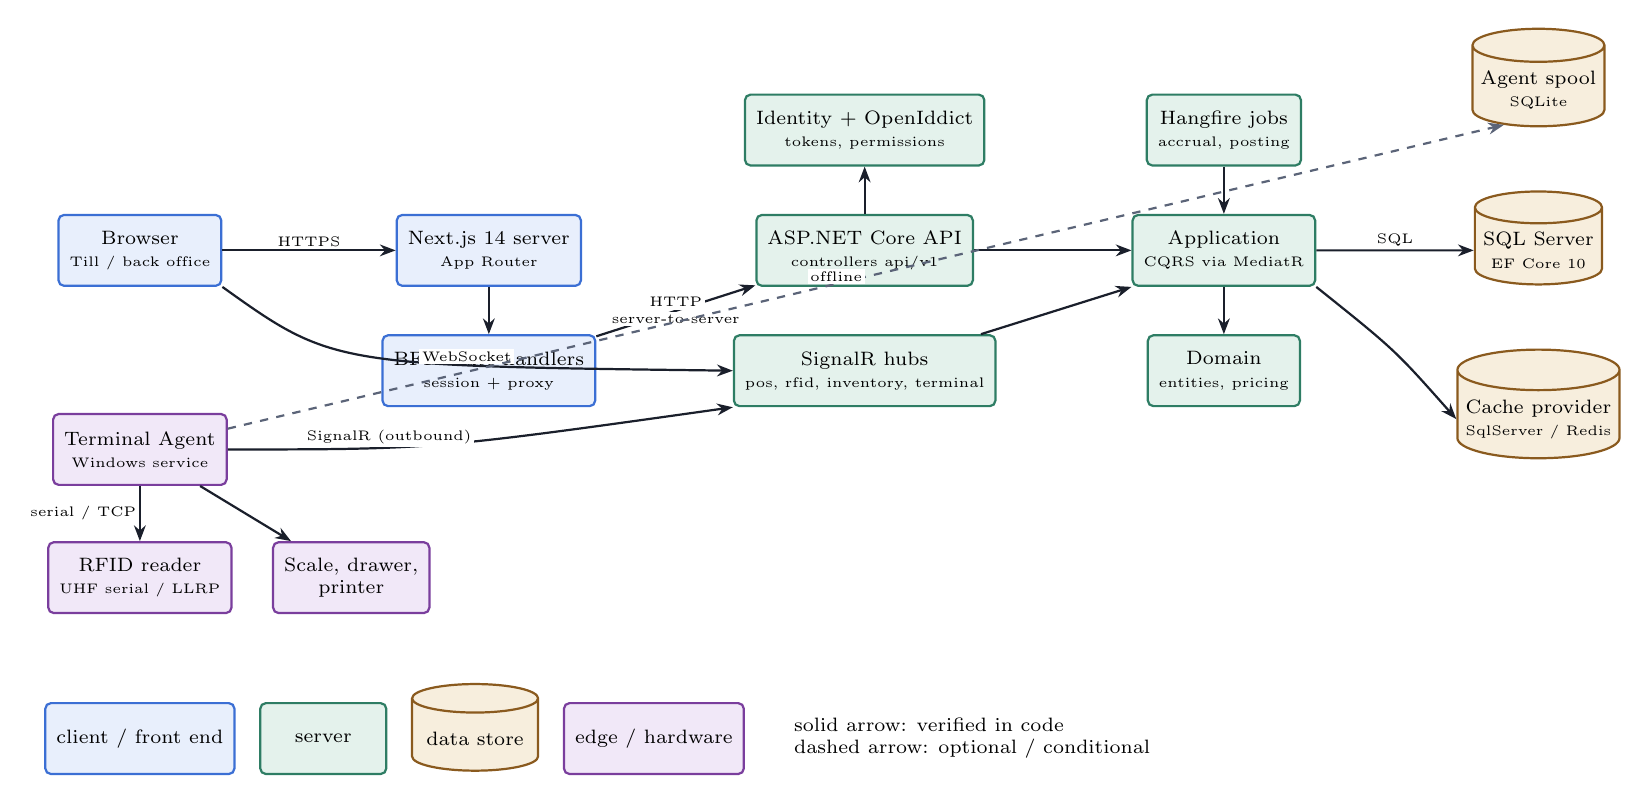
\begin{tikzpicture}[node distance=7mm]

% --- clients
\node[front] (browser) {Browser\\\tiny Till / back office};
\node[edge, below=16mm of browser] (agent) {Terminal Agent\\\tiny Windows service};
\node[edge, below=7mm of agent] (reader) {RFID reader\\\tiny UHF serial / LLRP};
\node[edge, right=5mm of reader] (periph) {Scale, drawer,\\printer};

% --- frontend
\node[front, right=22mm of browser] (next) {Next.js 14 server\\\tiny App Router};
\node[front, below=6mm of next] (bff) {BFF route handlers\\\tiny session + proxy};

% --- api
\node[back, right=22mm of next] (api) {ASP.NET Core API\\\tiny controllers api/v1};
\node[back, below=6mm of api] (hubs) {SignalR hubs\\\tiny pos, rfid, inventory, terminal};
\node[back, above=6mm of api] (authsrv) {Identity + OpenIddict\\\tiny tokens, permissions};

% --- core
\node[back, right=20mm of api] (appl) {Application\\\tiny CQRS via MediatR};
\node[back, below=6mm of appl] (domain) {Domain\\\tiny entities, pricing};
\node[back, above=6mm of appl] (jobs) {Hangfire jobs\\\tiny accrual, posting};

% --- data
\node[data, right=20mm of appl] (sql) {SQL Server\\\tiny EF Core 10};
\node[data, below=8mm of sql] (cache) {Cache provider\\\tiny SqlServer / Redis};
\node[data, above=8mm of sql] (spool) {Agent spool\\\tiny SQLite};

% --- arrows
\draw[flow] (browser) -- node[lbl,above]{HTTPS} (next);
\draw[flow] (next) -- (bff);
\draw[flow] (bff) -- node[lbl,above]{HTTP} node[lbl,below]{server-to-server} (api);
\draw[flow] (browser.south east) .. controls +(14mm,-10mm) .. node[lbl,above,pos=0.7]{WebSocket} (hubs.west);
\draw[flow] (api) -- (appl);
\draw[flow] (appl) -- (domain);
\draw[flow] (appl) -- node[lbl,above]{SQL} (sql);
\draw[flow] (api) -- (authsrv);
\draw[flow] (hubs) -- (appl.south west);
\draw[flow] (jobs) -- (appl);
\draw[flow] (appl.south east) .. controls +(10mm,-8mm) .. (cache.west);
\draw[flow] (agent) -- node[lbl,left]{serial / TCP} (reader);
\draw[flow] (agent) -- (periph);
\draw[flow] (agent.east) .. controls +(26mm,0) .. node[lbl,above,pos=0.35]{SignalR (outbound)} (hubs.south west);
\draw[flowdash] (agent) -- node[lbl,left]{offline} (spool.south west);

% --- legend
\begin{scope}[shift={(0,-62mm)}]
  \node[front, minimum width=16mm] (l1) {client / front end};
  \node[back,  minimum width=16mm, right=3mm of l1] (l2) {server};
  \node[data,  minimum width=16mm, right=3mm of l2] (l3) {data store};
  \node[edge,  minimum width=16mm, right=3mm of l3] (l4) {edge / hardware};
  \node[right=5mm of l4, font=\scriptsize, align=left] (l5)
    {solid arrow: verified in code\\dashed arrow: optional / conditional};
\end{scope}

\end{tikzpicture}}
\caption[System architecture]{System architecture as found in the repository. The browser never
calls the API directly: it talks to the Next.js server, whose route handlers hold the session and
proxy onward. The terminal agent connects \emph{outbound}, so a till needs no inbound firewall rule.}
\label{fig:arch}
\end{figure}

\section{Notes on the diagram}

\begin{itemize}[leftmargin=*,itemsep=3pt]
  \item \textbf{The browser holds no token.} The session is an encrypted, \code{httpOnly} cookie
        written by the Next.js server (\pathx{frontend/src/lib/server/session.ts}). API calls go
        through \pathx{app/api/proxy/[\ldots path]/route.ts}, which attaches the token server-side.
  \item \textbf{SignalR is the exception to that rule}, and is handled deliberately: the browser
        is issued a \emph{single-use hub ticket} from \pathx{app/api/auth/hub-ticket/route.ts}
        rather than a bearer token, because a WebSocket handshake cannot carry an
        \code{Authorization} header.
  \item \textbf{The agent dials out.} It is a SignalR \emph{client} of \code{/hubs/terminal}.
  \item \textbf{The cache is pluggable.} \code{Cache:Provider} selects SQL~Server, Redis or
        in-memory; the dashed path reflects that Redis is opt-in.
\end{itemize}

% =====================================================================================
\chapter{Application Runtime Flow}
\label{ch:flow}

Figure~\ref{fig:flow} traces a request from the browser through the system. It reflects the
implemented path: the browser's own fetch goes to the Next.js server, not to the API.

\begin{figure}[H]
\centering
\resizebox{0.97\textwidth}{!}{%
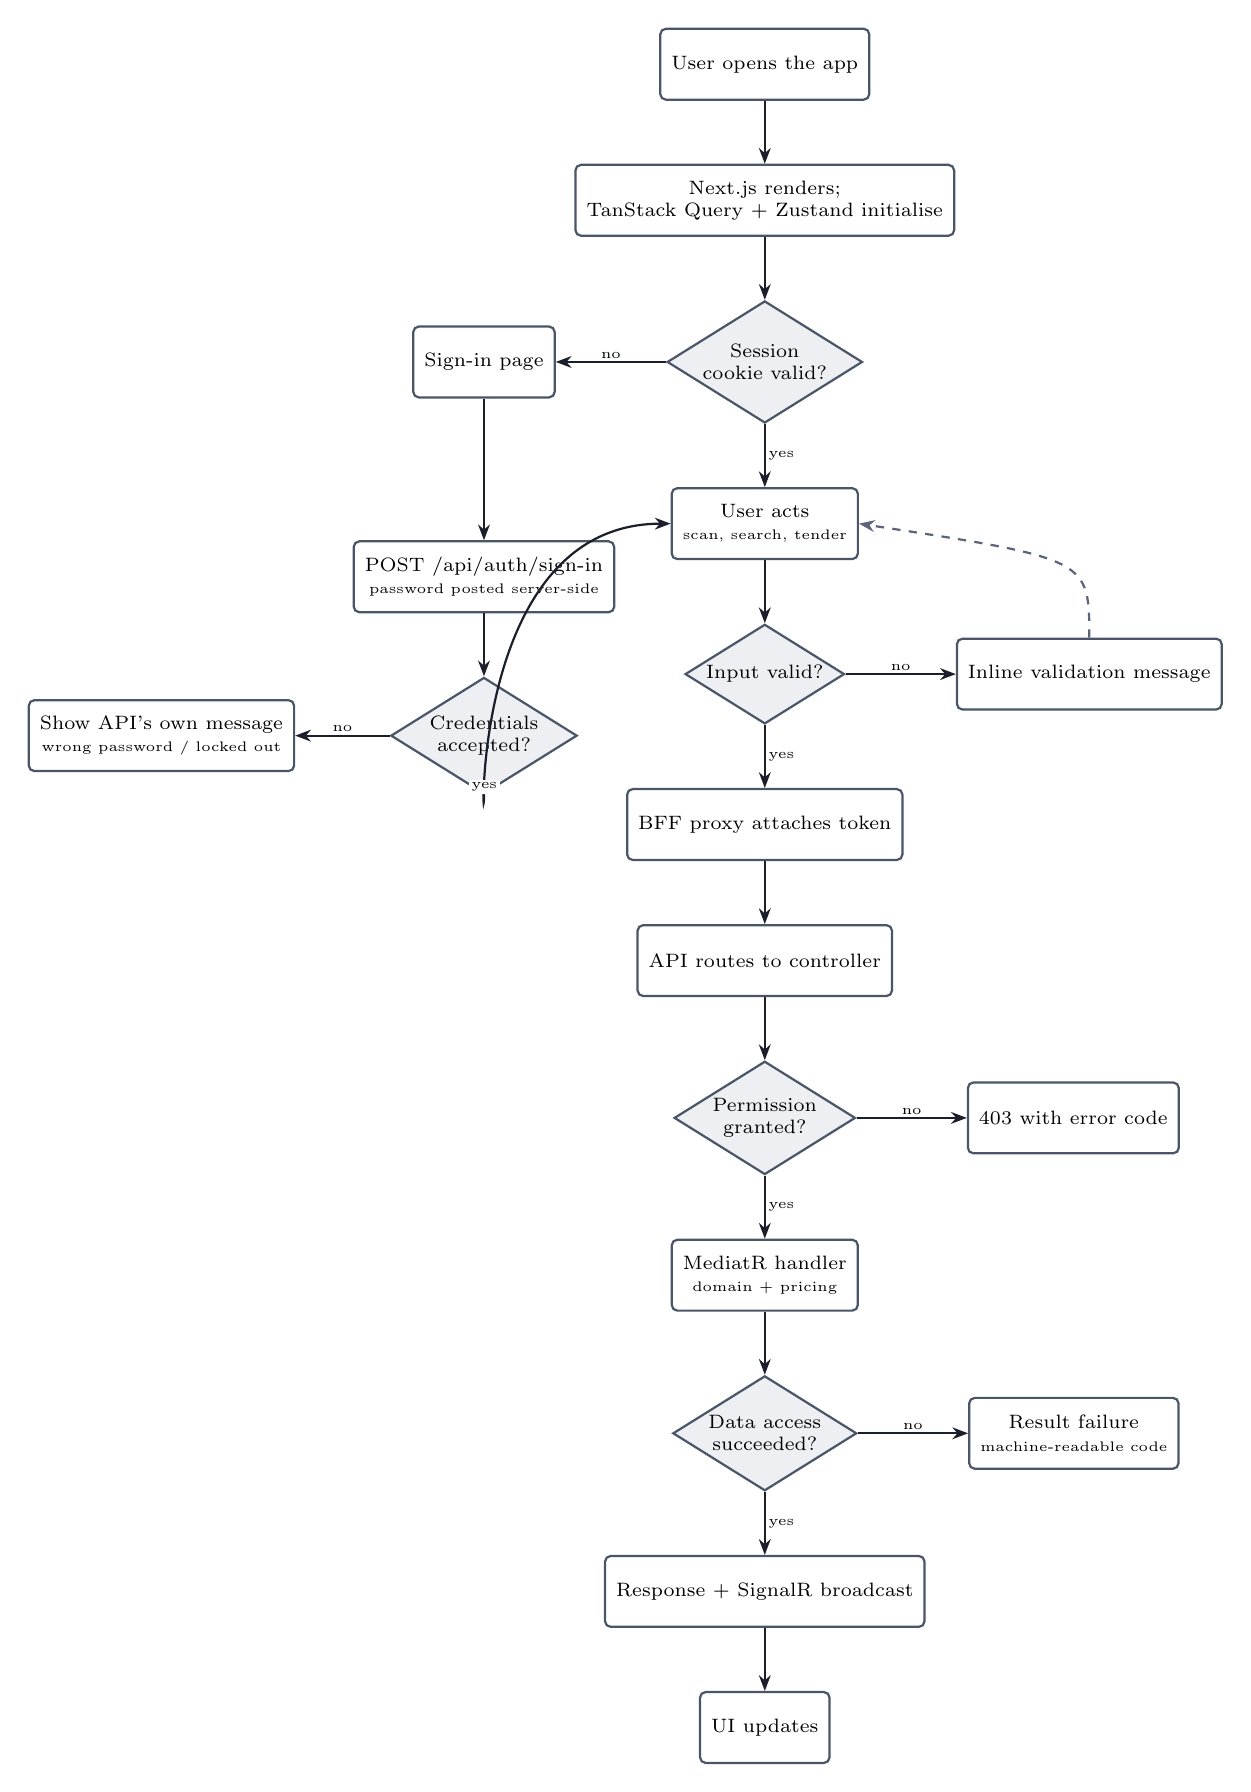
\begin{tikzpicture}[node distance=8mm]

\node[stage] (open) {User opens the app};
\node[stage, below=of open] (boot) {Next.js renders;\\TanStack Query + Zustand initialise};
\node[dec, below=of boot] (hassess) {Session\\cookie valid?};
\node[stage, left=14mm of hassess] (signin) {Sign-in page};
\node[stage, below=18mm of signin] (post) {POST /api/auth/sign-in\\\tiny password posted server-side};
\node[dec, below=of post] (credok) {Credentials\\accepted?};
\node[stage, left=12mm of credok] (autherr) {Show API's own message\\\tiny wrong password / locked out};

\node[stage, below=of hassess] (act) {User acts\\\tiny scan, search, tender};
\node[dec, below=of act] (valid) {Input valid?};
\node[stage, right=14mm of valid] (inperr) {Inline validation message};
\node[stage, below=of valid] (proxy) {BFF proxy attaches token};
\node[stage, below=of proxy] (route) {API routes to controller};
\node[dec, below=of route] (authz) {Permission\\granted?};
\node[stage, right=14mm of authz] (deny) {403 with error code};
\node[stage, below=of authz] (handler) {MediatR handler\\\tiny domain + pricing};
\node[dec, below=of handler] (dbok) {Data access\\succeeded?};
\node[stage, right=14mm of dbok] (fail) {Result failure\\\tiny machine-readable code};
\node[stage, below=of dbok] (ok) {Response + SignalR broadcast};
\node[stage, below=of ok] (ui) {UI updates};

\draw[flow] (open) -- (boot);
\draw[flow] (boot) -- (hassess);
\draw[flow] (hassess) -- node[lbl,above]{no} (signin);
\draw[flow] (signin) -- (post);
\draw[flow] (post) -- (credok);
\draw[flow] (credok) -- node[lbl,above]{no} (autherr);
\draw[flow] (credok.south) .. controls +(0,-8mm) and +(-26mm,0) .. node[lbl,below,pos=0.25]{yes} (act.west);
\draw[flow] (hassess) -- node[lbl,right]{yes} (act);
\draw[flow] (act) -- (valid);
\draw[flow] (valid) -- node[lbl,above]{no} (inperr);
\draw[flow] (valid) -- node[lbl,right]{yes} (proxy);
\draw[flow] (proxy) -- (route);
\draw[flow] (route) -- (authz);
\draw[flow] (authz) -- node[lbl,above]{no} (deny);
\draw[flow] (authz) -- node[lbl,right]{yes} (handler);
\draw[flow] (handler) -- (dbok);
\draw[flow] (dbok) -- node[lbl,above]{no} (fail);
\draw[flow] (dbok) -- node[lbl,right]{yes} (ok);
\draw[flow] (ok) -- (ui);
\draw[flowdash] (inperr.north) .. controls +(0,10mm) .. (act.east);

\end{tikzpicture}}
\caption[Application runtime flow]{Runtime flow for a browser-initiated action. Not every request
needs authorization or the database — read-only lookups short-circuit after the handler — so the
decision nodes are branches, not mandatory stages.}
\label{fig:flow}
\end{figure}

\section{The RFID path is different}

A tag read does not begin in the browser. The agent reads tags from the reader, debounces them
locally, and publishes them to \code{/hubs/terminal}. The server resolves which till the read
belongs to from the reader and antenna, prices it onto that till's cart, and notifies the till
over \code{/hubs/rfid}. The browser is a spectator in this path.

% =====================================================================================
\chapter{Frontend Technology}
\label{ch:frontend}

\section{Framework and rendering}

Next.js \textbf{14.2.35} (pinned exactly, not a range) using the \textbf{App Router}
(\pathx{frontend/src/app/}). \pathx{next.config.js} sets two options, both load-bearing:

\begin{itemize}[leftmargin=*,itemsep=2pt]
  \item \code{reactStrictMode: true} — React's development double-invoke is active.
  \item \code{output: 'standalone'} — emits \pathx{.next/standalone/server.js} with only the
        modules actually reached. The file's own comment gives the reason: shared hosting, where
        uploading a full \pathx{node\us modules} tree "is measured in hours".
\end{itemize}

\section{Screen inventory}

Routes under \pathx{src/app/(dashboard)/}: \code{admin}, \code{catalog}, \code{customers},
\code{dashboard}, \code{help}, \code{inventory}, \code{orders}, \code{pos}, \code{purchasing},
\code{receivables}, \code{reports}, \code{sales}. Outside the dashboard group:
\code{sign-in}, \code{sign-up}, \code{forgot-password}, \code{reset-password}, plus
\code{error.tsx}, \code{global-error.tsx} and \code{not-found.tsx} error boundaries.

\section{Layers}

\begin{small}
\begin{longtable}{L{3.4cm} L{3.6cm} L{7.88cm}}
\toprule
\textbf{Concern} & \textbf{Technology} & \textbf{Evidence} \\
\midrule
Server state & TanStack Query 5.101.4 & \pathx{package-lock.json}; devtools also present \\
Client state & Zustand 5.0.14 & \pathx{src/stores/pos-store.ts}, \pathx{ui-store.ts} \\
Styling & Tailwind CSS 3.4.19 + PostCSS 8.5.23 + Autoprefixer 10.5.4 & \pathx{tailwind.config.js}, \pathx{postcss.config.js} \\
Class composition & \code{clsx} 2.1.1, \code{tailwind-merge} 2.6.1, \code{class-variance-authority} 0.7.1 & \pathx{package.json} \\
Components & Radix UI primitives (dialog, dropdown-menu, label, select, separator, slot, tabs, toast, tooltip) & ten \code{@radix-ui/*} dependencies \\
Icons & \code{lucide-react} 0.468.0 & \pathx{package.json} \\
Charts & \code{recharts} 2.15.4 & \pathx{package.json} \\
Long lists & \code{@tanstack/react-virtual} 3.14.9 & used by the POS product grid \\
HTTP client & \code{axios} 1.18.1 & \pathx{src/lib/api-client.ts} \\
Realtime & \code{@microsoft/signalr} 8.0.17 & \pathx{src/lib/rfid-hub.ts}, \pathx{inventory-hub.ts} \\
Dates & \code{date-fns} 4.4.0 & \pathx{package.json} \\
Crypto (session seal) & \code{jose} 5.10.0 & \pathx{src/lib/server/session.ts} \\
\bottomrule
\end{longtable}
\end{small}

\section{Routing, forms and accessibility}

Routing is file-system based (App Router). \textbf{No dedicated form library} (React Hook Form,
Formik) and \textbf{no schema validation library} (Zod, Yup) is declared in
\pathx{package.json}; forms are handled with React state and server-side validation — recorded
here as \emph{Not Found} rather than assumed. Accessibility rests on Radix primitives, which
supply roles and keyboard behaviour; no separate accessibility tooling (axe, pa11y) is
configured.

% =====================================================================================
\chapter{Backend Technology}
\label{ch:backend}

\section{Runtime and host}

.NET~10 (\code{net10.0}), C\# \code{LangVersion 14.0}, with \code{Nullable} enabled and
\code{TreatWarningsAsErrors} set — so a warning fails the build. Analysers are on at
\code{latest-recommended}.

Entry point: \pathx{backend/src/Retail25.Api/Program.cs}. It configures, in order: Serilog
hosting, OpenTelemetry, health checks, controllers, Swagger, SignalR, CORS, authentication,
rate limiting, response compression, then the middleware pipeline and endpoint mapping.

\section{Project layout and dependency rule}

\begin{small}
\begin{longtable}{L{4.2cm} L{11.12cm}}
\toprule
\textbf{Project} & \textbf{Responsibility} \\
\midrule
\pathx{Retail25.Domain} & Entities, value objects, the pricing engine. No project references. \\
\pathx{Retail25.Application} & Commands, queries, handlers, ports. Depends on Domain and Contracts. \\
\pathx{Retail25.Infrastructure} & EF Core, Identity, OpenIddict, caching, realtime notifiers. Implements Application ports. \\
\pathx{Retail25.Api} & Controllers, SignalR hubs, host configuration. \\
\pathx{Retail25.Contracts} & Shared DTOs between server and agent. \\
\pathx{Retail25.Devices} & RFID and peripheral drivers (UHF serial, LLRP, simulator). \\
\pathx{Retail25.TerminalAgent} & Windows service running on a till. \\
\pathx{Retail25.Migration} & Legacy DBF and CSV importer. \\
\bottomrule
\end{longtable}
\end{small}

The direction of dependencies is enforced by a test, not only by convention:
\pathx{tests/Retail25.ArchitectureTests/DependencyRuleTests.cs} uses NetArchTest.

\section{Request handling}

Controllers are thin and dispatch through MediatR. Expected failures are returned as a
\code{Result} carrying a stable machine-readable code rather than thrown — visible throughout
the application layer and converted to HTTP status codes by a shared \code{ToActionResult}
extension.

\section{Cross-cutting services}

\begin{itemize}[leftmargin=*,itemsep=2pt]
  \item \textbf{Rate limiting} — three named policies in \pathx{Program.cs:305--307}:
        \code{auth} (20), \code{pin} (10) and \code{lookup} (300) per caller.
        \code{MapControllers().RequireRateLimiting("lookup")}.
  \item \textbf{Health checks} — \code{/health/live} and \code{/health/ready}
        (\pathx{Program.cs:415--416}), with SQL~Server and Redis checks registered.
  \item \textbf{Background jobs} — Hangfire, with two recurring jobs resolved from DI:
        \code{LateChargeAccrualJob} and \code{PostPosRevenueToAccountingJob}
        (\pathx{Program.cs:439--445}).
  \item \textbf{Response compression} and \textbf{Serilog request logging} are both enabled.
\end{itemize}

% =====================================================================================
\chapter{Programming Languages}
\label{ch:langs}

\begin{small}
\begin{longtable}{L{2.6cm} L{3.0cm} L{9.28cm}}
\toprule
\textbf{Language} & \textbf{Where} & \textbf{Evidence} \\
\midrule
C\# & All .NET projects & \pathx{*.csproj}; \code{LangVersion 14.0} in \pathx{Directory.Build.props} \\
TypeScript & All front-end source & \pathx{tsconfig.json}; \code{typescript} 5.9.3 locked \\
JavaScript & Build configuration & \pathx{next.config.js}, \pathx{tailwind.config.js}, \pathx{postcss.config.js} \\
SQL & Schema reference and diagnostics & \pathx{docs/architecture/schema.sql}, \pathx{docs/runbooks/diagnostic-queries.sql} \\
CSS & Global styles and Tailwind layers & \pathx{src/app/globals.css} \\
YAML & CI/CD and collector config & \pathx{.github/workflows/*.yml}, \pathx{deploy/otel/config.yaml}, \pathx{deploy/docker-compose.yml} \\
PowerShell & Operational scripts & \pathx{update-till-agent.ps1} and installer scripts \\
XML & Project and host configuration & \pathx{*.csproj}, \pathx{deploy/iis/frontend.web.config} \\
Dockerfile & Image definitions & \pathx{deploy/Dockerfile.api}, \pathx{deploy/Dockerfile.web} \\
\bottomrule
\end{longtable}
\end{small}

% =====================================================================================
\chapter{Frameworks}
\label{ch:frameworks}

\begin{small}
\begin{longtable}{L{3.2cm} L{1.9cm} L{9.78cm}}
\toprule
\textbf{Framework} & \textbf{Version} & \textbf{Role and configuration} \\
\midrule
ASP.NET Core & 10.0.x & API, hubs, health, rate limiting. Part of the shared framework; version tracks \code{net10.0}. \\
Entity Framework Core & 10.0.10 & ORM. SQL Server provider, snake-case naming via EFCore.NamingConventions 10.0.1, explicit migrations. \\
MediatR & 12.4.1 & CQRS dispatch. \\
FluentValidation & 11.11.0 & Request validation, with DI extensions. \\
OpenIddict & 7.6.0 & OAuth2/OIDC server. Pinned to 7.x because its EF Core integration binds to the EF Core major (comment in \pathx{Directory.Packages.props}). \\
ASP.NET Core Identity & 10.0.10 & Users, roles, lockout, password hashing. \\
Hangfire & 1.8.24 & Background jobs on SQL Server storage. \\
Next.js & 14.2.35 & React framework, App Router, standalone output. \\
React & 18.3.1 & UI rendering. \\
Tailwind CSS & 3.4.19 & Utility CSS. \\
xUnit & 2.9.3 & Test framework for all five test projects. \\
Playwright & 1.62.0 & End-to-end browser tests. \\
Vitest & 2.1.9 & Front-end unit tests (\code{environment: 'node'}). \\
\bottomrule
\end{longtable}
\end{small}

% =====================================================================================
\chapter{Libraries and Important Dependencies}
\label{ch:libs}

All .NET versions below come from \pathx{backend/Directory.Packages.props}, which uses Central
Package Management — every version is pinned exactly, so declared and effective versions are the
same. Front-end versions are the \emph{locked} versions from \pathx{frontend/package-lock.json}
(lockfile version~3).

\section{Backend, by purpose}

\begin{small}
\begin{longtable}{L{4.6cm} L{2.0cm} L{7.6cm}}
\caption{Backend dependencies by purpose}\label{tab:backendlibs}\\
\toprule
\textbf{Package} & \textbf{Version} & \textbf{Why it is here} \\
\midrule
\endfirsthead
\toprule
\textbf{Package} & \textbf{Version} & \textbf{Why it is here} \\
\midrule
\endhead
\midrule \multicolumn{3}{r}{\small\itshape continued on next page}\\
\endfoot
\bottomrule
\endlastfoot

\multicolumn{3}{l}{\textit{Application core}}\\
MediatR & 12.4.1 & Command/query dispatch \\
FluentValidation (+ DI ext.) & 11.11.0 & Request validation \\
Mapster & 7.4.0 & Object mapping \\
\addlinespace
\multicolumn{3}{l}{\textit{Persistence}}\\
\pkg{Microsoft.EntityFrameworkCore} & 10.0.10 & ORM core \\
\quad .Relational / .SqlServer / .Design & 10.0.10 & Provider and migration tooling \\
\quad .InMemory & 10.0.10 & Test provider \\
\pkg{EFCore.NamingConventions} & 10.0.1 & snake\us case table and column names \\
\pkg{Microsoft.Data.Sqlite} & 10.0.10 & The agent's offline tag spool \\
\addlinespace
\multicolumn{3}{l}{\textit{Identity and security}}\\
\pkg{Identity.EntityFrameworkCore} & 10.0.10 & User and role stores \\
\pkg{DataProtection.EntityFrameworkCore} & 10.0.10 & Keys persisted to the database, so they survive a recycle \\
\pkg{Authentication.JwtBearer} & 10.0.10 & Staff and shopper bearer schemes \\
\pkg{OpenIddict.AspNetCore} & 7.6.0 & Authorization and token endpoints \\
\pkg{OpenIddict.EntityFrameworkCore} & 7.6.0 & Client and token storage \\
\pkg{OpenIddict.Validation.AspNetCore} & 7.6.0 & Token validation \\
Konscious\ldots Argon2 & 1.3.1 & PIN hashing \\
\addlinespace
\multicolumn{3}{l}{\textit{Caching and realtime}}\\
\pkg{StackExchange.Redis} & 2.8.16 & Redis client (opt-in) \\
\pkg{SignalR.StackExchangeRedis} & 10.0.10 & Hub backplane when Redis is used \\
\pkg{SignalR.Client} & 10.0.10 & Used by the terminal agent \\
\addlinespace
\multicolumn{3}{l}{\textit{Jobs, documents, data}}\\
Hangfire.AspNetCore / .SqlServer & 1.8.24 & Recurring jobs \\
QuestPDF & 2024.10.3 & Receipts and PDF documents \\
\pkg{ZXing.Net} & 0.16.9 & Barcode encoding/decoding \\
ClosedXML & 0.104.2 & Excel export \\
CsvHelper & 33.0.1 & CSV import/export \\
YamlDotNet & 16.2.1 & YAML parsing \\
\addlinespace
\multicolumn{3}{l}{\textit{Observability}}\\
\pkg{Serilog.AspNetCore} & 10.0.0 & Structured logging \\
Serilog sinks: Console / File & 6.1.1 / 7.0.0 & Log destinations \\
\pkg{OpenTelemetry.Extensions.Hosting} & 1.17.0 & Telemetry host integration \\
OTLP exporter; ASP.NET Core, Http, Runtime instrumentation & 1.17.0 & Traces and metrics \\
\addlinespace
\multicolumn{3}{l}{\textit{API surface}}\\
\pkg{Swashbuckle.AspNetCore} & 10.2.3 & Swagger/OpenAPI \\
\pkg{Microsoft.AspNetCore.OpenApi} & 10.0.10 & OpenAPI metadata \\
HealthChecks.SqlServer / .Redis & 9.0.0 & Readiness probes \\
\addlinespace
\multicolumn{3}{l}{\textit{Hardware}}\\
\pkg{System.IO.Ports} & 10.0.10 & Serial access for readers and peripherals \\
\pkg{Hosting.WindowsServices} & 10.0.10 & Runs the agent as a Windows service \\
\end{longtable}
\end{small}

\section{Security pins}

\pathx{Directory.Packages.props} carries a block of transitive pins that exist solely to clear
advisories, each annotated in the file with its GHSA identifier:

\begin{small}
\begin{longtable}{L{5.4cm} L{1.8cm} L{7.68cm}}
\toprule
\textbf{Package} & \textbf{Pinned} & \textbf{Advisory / arrives via} \\
\midrule
Newtonsoft.Json & 13.0.3 & GHSA-5crp-9r3c-p9vr; under Hangfire \\
SQLitePCLRaw (lib, bundle, core, provider) & 2.1.12 & GHSA-2m69-gcr7-jv3q; under Microsoft.Data.Sqlite \\
MessagePack & 2.5.302 & GHSA-4qm4-8hg2-g2xm; SignalR hub protocol \\
\bottomrule
\end{longtable}
\end{small}

The file records the reasoning: each is pinned to the lowest patched version \emph{inside its
existing major}, because taking the newest would mean major bumps "across a serial-port spool and
a hub protocol, for no security benefit over these."

% =====================================================================================
\chapter{Database and Data Layer}
\label{ch:data}

\section{Engine and access}

\begin{small}
\begin{longtable}{L{4.2cm} L{11.12cm}}
\toprule
\textbf{Aspect} & \textbf{Finding} \\
\midrule
Engine & Microsoft SQL Server. \code{UseSqlServer} at \pathx{Infrastructure/DependencyInjection.cs:83} \\
Container image & \code{mcr.microsoft.com/mssql/server:2022-latest} (\pathx{deploy/docker-compose.yml}) \\
ORM & EF Core 10.0.10 \\
Naming & snake\us case via \code{UseSnakeCaseNamingConvention()} \\
Context & \code{ApplicationDbContext}, \textbf{89} \code{DbSet} properties \\
Configurations & 28 files in \pathx{Persistence/Configurations/} \\
Migrations & 12, latest \code{20260819081314\us DeviceEnrolment} \\
Applied & On start when \code{Database:AutoMigrate} is set \\
Design-time & \code{DesignTimeDbContextFactory} for \code{dotnet ef} \\
Secondary store & SQLite (\code{Microsoft.Data.Sqlite}) — the agent's offline tag spool \\
\bottomrule
\end{longtable}
\end{small}

\section{Domain areas}

\pathx{Retail25.Domain} is organised by aggregate area: \code{Accounting}, \code{Catalog},
\code{Common}, \code{Configuration}, \code{Customers}, \code{Identification}, \code{Inventory},
\code{Migration}, \code{Orders}, \code{Purchasing}, \code{Receivables}, \code{Sales},
\code{Security}, \code{Shoppers}, \code{Staff}, \code{Terminals}, \code{Trolleys},
\code{ValueObjects}.

\section{The ledger decision}

\pathx{README.md} states the governing rule: \emph{"The transaction is a ledger, not a row."}
Sales, stock movements, AR balances and drawer totals are append-only, with derived snapshots —
\code{Product.OnHand} is a projection of \code{stock\us ledger\us entries} rather than an
independently mutated number. The README attributes this to the legacy system's DBF mutation and
its need for \code{Rebuild}/\code{Reindex} recovery.

A full entity-relationship diagram is not reproduced here: with 89 entity sets it would be
unreadable at page size, and a generated reference already exists at
\pathx{docs/architecture/schema.sql} and \pathx{docs/architecture/12-schema-reference.md}.
Figure~\ref{fig:rfidmodel} shows the one sub-model that this document's RFID discussion depends on.

\begin{figure}[H]
\centering
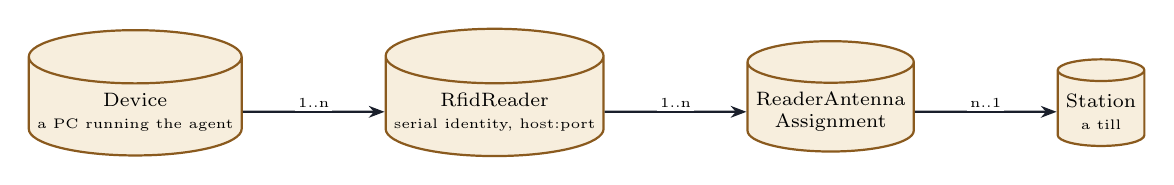
\begin{tikzpicture}[node distance=12mm]
\node[data] (device) {Device\\\tiny a PC running the agent};
\node[data, right=18mm of device] (reader) {RfidReader\\\tiny serial identity, host:port};
\node[data, right=18mm of reader] (assign) {ReaderAntenna\\Assignment};
\node[data, right=18mm of assign] (station) {Station\\\tiny a till};
\draw[flow] (device) -- node[lbl,above]{1..n} (reader);
\draw[flow] (reader) -- node[lbl,above]{1..n} (assign);
\draw[flow] (assign) -- node[lbl,above]{n..1} (station);
\end{tikzpicture}
\caption[RFID topology model]{The RFID topology sub-model. One machine drives many readers; each
reader's antennas are mapped individually to tills, so one four-antenna reader can serve four
separate checkouts. Introduced by migration \code{20260819071121\us RfidTopology}.}
\label{fig:rfidmodel}
\end{figure}

\section{Secrets}

No connection string, password or key is reproduced in this document. Connection strings are
supplied through configuration (\code{ConnectionStrings:DefaultConnection}); the deployment
workflow injects the staff token signing key as a secret at publish time.

% =====================================================================================
\chapter{Authentication and Authorization}
\label{ch:auth}

\section{What is actually implemented}

This is the area where the project's documentation and its code diverge most, so the findings are
stated plainly with evidence.

\begin{small}
\begin{longtable}{L{3.6cm} L{11.72cm}}
\toprule
\textbf{Audience} & \textbf{Mechanism} \\
\midrule
Staff (till, back office) & \textbf{Custom JWT endpoint.} \code{POST /auth/token} in
\pathx{StaffAuthController.cs:74}. Credentials are checked with ASP.NET Core Identity's
\code{CheckPasswordSignInAsync(\ldots, lockoutOnFailure: true)} (line 96) and a token pair is
issued by \code{StaffTokenIssuer}. Also \code{POST /auth/refresh} and \code{GET /auth/me}. \\
Shopper (phone app) & Separate \code{JwtBearer} scheme, \code{ShopperAuthentication.Scheme}
(\pathx{IdentityRegistration.cs:319}), with its own signing key and no permission claims. \\
Machine clients (terminal agent) & OpenIddict \code{client\us credentials} against
\code{connect/token}. \\
\bottomrule
\end{longtable}
\end{small}

OpenIddict is configured with \code{AllowAuthorizationCodeFlow()},
\code{AllowRefreshTokenFlow()} and \code{AllowClientCredentialsFlow()}
(\pathx{IdentityRegistration.cs:161--163}), exposing \code{connect/authorize} and
\code{connect/token}. The authorization-code flow therefore \emph{exists}; it is simply not what
staff sign-in uses any more. \pathx{frontend/src/app/api/auth/sign-in/route.ts} records the move
in its own comment: the password "is posted to the API from the server", which keeps the
"no token is reachable from JavaScript" guarantee "true after moving off the redirect flow".

\section{Session handling in the browser}

\begin{itemize}[leftmargin=*,itemsep=2pt]
  \item One cookie, written by the Next.js server: \code{httpOnly}, \code{SameSite=Lax}, and
        \code{Secure} in production.
  \item Named \code{\us\us Host-r25.session} in production and \code{r25.session} otherwise.
        The code explains the split: the \code{\us\us Host-} prefix requires \code{Secure}, which
        plain-HTTP development cannot satisfy, and a browser silently discards a prefixed cookie
        that fails the contract.
  \item Contents are sealed with \code{jose} 5.10.0 before being written.
  \item Data Protection keys are persisted to the database
        (\code{DataProtection.EntityFrameworkCore}), so an application-pool recycle does not
        invalidate every session.
\end{itemize}

\section{Authorization}

Permissions are data, not code: \code{permission} and \code{role\us permission} rows resolved by
a \code{PermissionResolver}, with a \code{PermissionClaim} carried on the identity. Hub access
uses a dedicated policy (\code{HubAuthorizationPolicy}) that requires an authenticated user.
PINs are hashed with Argon2 (\code{Argon2PinHasher}).

\begin{figure}[H]
\centering
\resizebox{0.95\textwidth}{!}{%
\begin{tikzpicture}[node distance=8mm]
\node[stage] (a) {Browser posts username + password\\to \code{/api/auth/sign-in}};
\node[stage, below=of a] (b) {Next.js server calls API \code{/auth/token}};
\node[dec, below=of b] (c) {User found?};
\node[stage, right=16mm of c] (c2) {401 — API's own wording};
\node[dec, below=of c] (d) {Password ok\\and not locked out?};
\node[stage, below=of d] (e) {\code{StaffTokenIssuer} mints\\access + refresh tokens};
\node[stage, below=of e] (f) {Server seals them into the\\session cookie (httpOnly)};
\node[stage, below=of f] (g) {Browser holds a cookie\\and no token};
\node[dec, below=of g] (h) {Access token\\expired?};
\node[stage, right=16mm of h] (i) {Server calls \code{/auth/refresh}};
\node[stage, below=of h] (j) {Proxy attaches token\\to each API call};
\node[dec, below=of j] (k) {Permission\\satisfied?};
\node[stage, right=16mm of k] (l) {403 with error code};
\node[stage, below=of k] (m) {Handler runs};

\draw[flow] (a) -- (b);
\draw[flow] (b) -- (c);
\draw[flow] (c) -- node[lbl,above]{no} (c2);
\draw[flow] (c) -- node[lbl,right]{yes} (d);
\draw[flow] (d) -- node[lbl,right]{yes} (e);
\draw[flow] (d.west) .. controls +(-14mm,0) and +(-14mm,0) .. node[lbl,left]{no} (c2.west);
\draw[flow] (e) -- (f);
\draw[flow] (f) -- (g);
\draw[flow] (g) -- (h);
\draw[flow] (h) -- node[lbl,above]{yes} (i);
\draw[flow] (i.south) .. controls +(0,-10mm) .. (j.east);
\draw[flow] (h) -- node[lbl,right]{no} (j);
\draw[flow] (j) -- (k);
\draw[flow] (k) -- node[lbl,above]{no} (l);
\draw[flow] (k) -- node[lbl,right]{yes} (m);
\end{tikzpicture}}
\caption[Authentication and authorization flow]{Staff authentication and authorization.
Authentication establishes identity at the token endpoint; authorization is a separate
permission check on each API call.}
\label{fig:auth}
\end{figure}

\section{The hub ticket}

A WebSocket handshake cannot carry an \code{Authorization} header, and handing the browser a
bearer token would defeat the backend-for-frontend. The system issues a \emph{single-use hub
ticket} instead (\pathx{app/api/auth/hub-ticket/route.ts} $\rightarrow$
\code{api/v1/hub-tickets}), redeemed by \code{HubTicketMiddleware} and exchanged for a
claims identity. The route's own comment describes the ticket as "deliberately almost worthless:
it authenticates one hub connection, expires in a minute, and is consumed on use."

% =====================================================================================
\chapter{API Technology}
\label{ch:api}

\section{Style and shape}

A REST-style HTTP API of ASP.NET Core controllers, versioned by path segment
(\code{api/v1/\ldots}), alongside four SignalR hubs for realtime. OpenAPI is produced by
Swashbuckle 10.2.3 (\code{SwaggerDoc("v1", \ldots Title = "Retail25 API")},
\pathx{Program.cs:98}).

\section{Endpoint groups}

Forty route prefixes were found. Grouped by area:

\begin{small}
\begin{longtable}{L{3.2cm} L{12.12cm}}
\toprule
\textbf{Area} & \textbf{Route prefixes under \code{api/v1/}} \\
\midrule
Selling & \code{carts}, \code{sales}, \code{price-quotes}, \code{tender-types}, \code{drawer-sessions}, \code{layaways}, \code{customer-orders}, \code{gift-cards} \\
Catalogue \& stock & \code{catalog}, \code{catalog/bulk}, \code{products}, \code{products/\{id\}/matrix}, \code{inventory}, \code{stock-counts}, \code{transfers}, \code{serialized-units} \\
Purchasing \& finance & \code{purchase-orders}, \code{suppliers}, \code{receivables}, \code{fiscal-years}, \code{sync/accounting} \\
People & \code{customers}, \code{staff}, \code{loyalty}, \code{account}, \code{approvals} \\
Hardware & \code{terminals}, \code{rfid-topology}, \code{hub-tickets} \\
Shopper app & \code{shopper}, \code{shopper/account} \\
Platform & \code{settings}, \code{reports}, \code{documents}, \code{audit}, \code{diagnostics}, \code{maintenance}, \code{migration}, \code{locations/\{id\}/branding} \\
Outside \code{api/v1} & \code{auth} (staff tokens), \code{account} (interactive pages), \code{connect/*} (OpenIddict) \\
\bottomrule
\end{longtable}
\end{small}

\section{Realtime hubs}

\begin{small}
\begin{longtable}{L{3.0cm} L{12.32cm}}
\toprule
\textbf{Hub} & \textbf{Purpose} \\
\midrule
\code{/hubs/pos} & Till state and sale updates \\
\code{/hubs/inventory} & Back-office grid patches \\
\code{/hubs/terminal} & The agent's own channel (tags in, commands out) \\
\code{/hubs/rfid} & Tag observations and reader status to the till \\
\bottomrule
\end{longtable}
\end{small}

\section{Conventions}

Errors return a problem document with a stable \code{code} (for example
\code{device.not\us found}, \code{validation.failed}) rather than an English sentence, so the UI
can translate. Rate limiting is applied per caller with the three policies named in
Chapter~\ref{ch:backend}. CORS exposes a single named policy, \code{Frontend}, whose origins come
from \code{AllowedOrigins}.

\begin{figure}[H]
\centering
\resizebox{0.98\textwidth}{!}{%
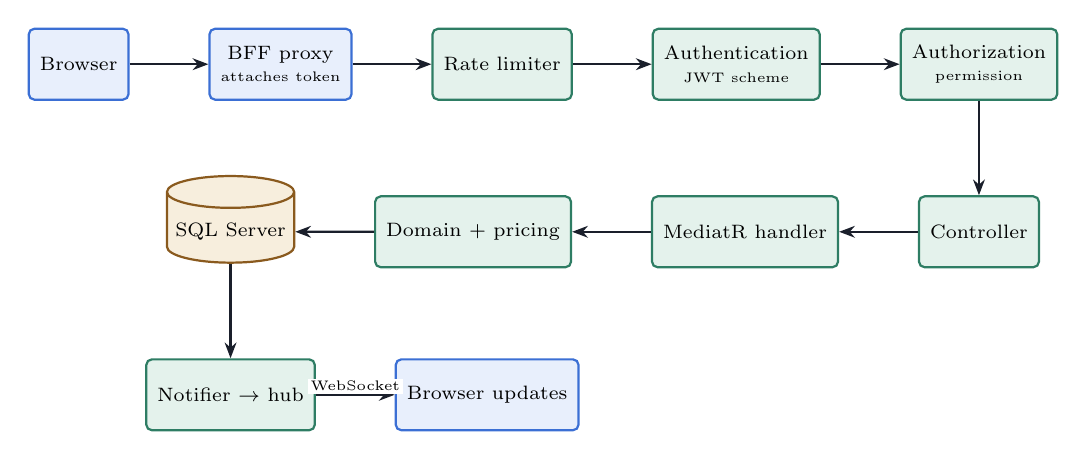
\begin{tikzpicture}[node distance=10mm]
\node[front] (b) {Browser};
\node[front, right=of b] (p) {BFF proxy\\\tiny attaches token};
\node[back, right=of p] (rl) {Rate limiter};
\node[back, right=of rl] (au) {Authentication\\\tiny JWT scheme};
\node[back, right=of au] (az) {Authorization\\\tiny permission};
\node[back, below=12mm of az] (ct) {Controller};
\node[back, left=of ct] (md) {MediatR handler};
\node[back, left=of md] (dm) {Domain + pricing};
\node[data, left=of dm] (db) {SQL Server};
\node[back, below=12mm of db] (nt) {Notifier $\rightarrow$ hub};
\node[front, right=of nt] (ui) {Browser updates};

\draw[flow] (b) -- (p); \draw[flow] (p) -- (rl); \draw[flow] (rl) -- (au);
\draw[flow] (au) -- (az); \draw[flow] (az) -- (ct); \draw[flow] (ct) -- (md);
\draw[flow] (md) -- (dm); \draw[flow] (dm) -- (db); \draw[flow] (db) -- (nt);
\draw[flow] (nt) -- node[lbl,above]{WebSocket} (ui);
\end{tikzpicture}}
\caption[API request lifecycle]{Lifecycle of an API request, from the browser through the
backend-for-frontend proxy to the database, and the realtime notification that follows a
state change.}
\label{fig:apiflow}
\end{figure}

% =====================================================================================
\chapter{Build Tools and Package Management}
\label{ch:build}

\begin{small}
\begin{longtable}{L{3.6cm} L{3.4cm} L{7.88cm}}
\toprule
\textbf{Concern} & \textbf{Tool} & \textbf{Evidence} \\
\midrule
.NET package manager & NuGet, \emph{Central Package Management} & \pathx{Directory.Packages.props}, \code{ManagePackageVersionsCentrally}, \code{CentralPackageTransitivePinningEnabled} \\
.NET build & \code{dotnet build} / \code{dotnet publish} & \pathx{Retail25.sln}; CI and deploy workflows \\
.NET compiler settings & \code{net10.0}, C\# 14, warnings as errors & \pathx{Directory.Build.props} \\
Node package manager & npm & \pathx{package-lock.json}, lockfile version 3; CI uses \code{npm ci} \\
Front-end build & \code{next build} (standalone output) & \pathx{package.json} scripts; \pathx{next.config.js} \\
Dev server & \code{next dev} & \pathx{package.json} \\
Type checking & \code{tsc --noEmit} & \code{typecheck} script \\
Linting & ESLint 8.57.1 + \code{eslint-config-next} 14.2.21 & \code{lint} script \\
CSS pipeline & PostCSS 8.5.23, Autoprefixer 10.5.4, Tailwind 3.4.19 & \pathx{postcss.config.js} \\
\bottomrule
\end{longtable}
\end{small}

No .NET-side formatter configuration (\pathx{.editorconfig} aside) and no Prettier configuration
were found; code formatting for the front end rests on ESLint. Recorded as \emph{Not Found}.

% =====================================================================================
\chapter{Testing}
\label{ch:testing}

\section{What exists}

\begin{small}
\begin{longtable}{L{4.6cm} L{1.8cm} L{8.48cm}}
\toprule
\textbf{Project / suite} & \textbf{Files} & \textbf{Kind and tooling} \\
\midrule
\pathx{Retail25.Domain.UnitTests} & 15 & Pricing and tax. Property-based testing with CsCheck 4.2.0. \\
\pathx{Retail25.Application.UnitTests} & 52 & Handler and service behaviour; NSubstitute 5.3.0 for doubles. \\
\pathx{Retail25.TerminalAgent.UnitTests} & 16 & Agent, codecs, spool. \\
\pathx{Retail25.ArchitectureTests} & 2 & Dependency rules (NetArchTest 1.3.2) and shipped transport-security settings. \\
\pathx{Retail25.IntegrationTests} & 24 & Real SQL Server and Redis via Testcontainers 4.0.0; \code{Mvc.Testing} for in-process hosting. \\
\pathx{frontend} unit & — & Vitest 2.1.9, \code{environment: 'node'}, \code{src/**/*.test.ts(x)}. \\
\pathx{frontend/e2e} & 5 specs & Playwright 1.62.0 against a running stack. \\
\bottomrule
\end{longtable}
\end{small}

Coverage collection is available through \code{coverlet.collector} 6.0.2. Static analysis is the
.NET analyser set at \code{latest-recommended} with warnings as errors, plus ESLint on the front
end.

\section{Configured versus executed}

Everything above is \emph{configured}. This document makes no claim about current pass rates:
no test run was performed as part of generating it, and CI results are not reproduced here.
A reviewer wanting that evidence should consult the most recent run of
\pathx{.github/workflows/ci.yml}.

\section{A gap worth recording}

\pathx{CLAUDE.md} (present on another branch, see Chapter~\ref{ch:evidence}) describes a
\emph{parity benchmark} of 155 legacy behaviours, generated into \pathx{docs/BENCHMARK.md} and
driven by \pathx{Benchmark/capabilities.json}. \textbf{Neither file exists on this branch}, and
\pathx{Retail25.ArchitectureTests} contains only the two suites listed above. The parity-tracking
mechanism described in that document is therefore \emph{Not Found} here.

% =====================================================================================
\chapter{Deployment and CI/CD}
\label{ch:deploy}

\section{Continuous integration}

\pathx{.github/workflows/ci.yml} defines four jobs: \code{backend}, \code{frontend},
\code{e2e} and \code{containers}. The backend job restores, builds with warnings as errors,
runs the unit, agent and architecture suites, then the integration suite, and asserts that the
integration suite actually executed rather than skipping. The \code{e2e} job starts SQL Server
and Redis as services, generates throwaway token-signing keys, starts the API, installs
Playwright and runs the browser suite. The \code{containers} job builds both images and pushes
them to GHCR only from \code{main}.

\section{Release pipeline}

\pathx{.github/workflows/deploy-myasp.yml} targets shared Windows hosting and defines five jobs:
\code{test}, \code{backend}, \code{frontend}, \code{database} and \code{deploy}. Notable steps
visible in the file: restoring a hand-maintained \pathx{web.config}, injecting the staff token
signing key as a secret, and proving the sub-application configuration and the assembled
front-end tree are intact before publishing.

\begin{figure}[H]
\centering
\resizebox{\textwidth}{!}{%
\begin{tikzpicture}[node distance=9mm]
\node[stage] (src) {Push to \code{main}};
\node[stage, right=of src] (test) {\code{test}\\\tiny backend tests, FE typecheck + lint};
\node[stage, right=of test] (be) {\code{backend}\\\tiny publish API, inject signing key};
\node[stage, below=12mm of be] (fe) {\code{frontend}\\\tiny npm ci, next build, assemble tree};
\node[stage, left=of fe] (dbj) {\code{database}\\\tiny EF tooling, apply migrations};
\node[stage, left=of dbj] (dep) {\code{deploy}\\\tiny Web Deploy to host};
\node[infra, below=12mm of dep] (live) {pos.sma-techno.net};

\draw[flow] (src) -- (test);
\draw[flow] (test) -- (be);
\draw[flow] (be) -- (fe);
\draw[flow] (fe) -- (dbj);
\draw[flow] (dbj) -- (dep);
\draw[flow] (dep) -- (live);
\end{tikzpicture}}
\caption[Release pipeline]{The release pipeline to shared Windows hosting. Job names are taken
verbatim from \pathx{.github/workflows/deploy-myasp.yml}; the arrows show the order in which the
file declares them and should not be read as a guarantee of strict sequencing.}
\label{fig:deploy}
\end{figure}

\section{Container and host options}

\begin{small}
\begin{longtable}{L{3.6cm} L{11.72cm}}
\toprule
\textbf{Artefact} & \textbf{Content} \\
\midrule
\pathx{deploy/Dockerfile.api} & Build on \code{mcr.microsoft.com/dotnet/sdk:10.0}; run on \code{aspnet:10.0}; \code{EXPOSE 8080}; entrypoint \code{dotnet Retail25.Api.dll} \\
\pathx{deploy/Dockerfile.web} & Three stages on \code{node:20-alpine}; \code{EXPOSE 3000}; \code{CMD ["node","server.js"]} (standalone output) \\
\pathx{deploy/docker-compose.yml} & Services \code{sqlserver} (\code{mssql/server:2022-latest}), \code{redis} (\code{redis:7-alpine}), \code{otel-collector} (\code{otel/opentelemetry-collector-contrib:0.115.1}), \code{api}, \code{web}; volumes \code{sqldata}, \code{redisdata} \\
\pathx{deploy/caddy/Caddyfile} & Reverse proxy configuration \\
\pathx{deploy/iis/frontend.web.config} & IIS host configuration for the front end \\
\pathx{deploy/otel/config.yaml} & Collector pipeline \\
\bottomrule
\end{longtable}
\end{small}

\section{The terminal agent is not part of either pipeline}

The agent is installed on a till by hand and is not produced or deployed by CI. It is a Windows
service (\code{Hosting.WindowsServices}) with \code{StartType=Automatic} and failure-restart
actions, and it connects outbound, so a till needs no inbound firewall rule.

% =====================================================================================
\chapter{Hosting Requirements}
\label{ch:hosting}

Each requirement carries a label: \vok{} established by a project file; \vder{} reasonably
inferred from the implementation; \vrec{} a proposed practice, not a project requirement;
\vno{} insufficient evidence.

\begin{small}
\begin{longtable}{L{4.2cm} L{2.6cm} L{7.2cm}}
\caption{Hosting and runtime requirements}\label{tab:hosting}\\
\toprule
\textbf{Requirement} & \textbf{Status} & \textbf{Detail and evidence} \\
\midrule
\endfirsthead
\toprule
\textbf{Requirement} & \textbf{Status} & \textbf{Detail and evidence} \\
\midrule
\endhead
\midrule \multicolumn{3}{r}{\small\itshape continued on next page}\\
\endfoot
\bottomrule
\endlastfoot

.NET runtime & \vok & ASP.NET Core 10 runtime; \code{net10.0} in \pathx{Directory.Build.props} \\
Node runtime & \vok & Node 20 for the front end; \code{node:20-alpine} in \pathx{Dockerfile.web} \\
Database & \vok & SQL Server; image \code{mssql/server:2022-latest} in Compose \\
Redis & \vok & Optional. Only when \code{Cache:Provider} is Redis; \code{redis:7-alpine} \\
API port & \vok & 8080 in the container (\code{EXPOSE 8080}) \\
Web port & \vok & 3000 in the container (\code{EXPOSE 3000}) \\
HTTPS & \vok & A startup guard refuses to run with the shipped placeholder public origin; \code{\us\us Host-} cookies require \code{Secure} \\
Public origin configuration & \vok & \code{Auth:WebOrigin} and \code{AllowedOrigins} must be set, or the API refuses to start \\
Token signing keys & \vok & Outside Development, OpenIddict refuses to start without signing and encryption certificates \\
Database migration on start & \vok & Applied when \code{Database:AutoMigrate} is set \\
Windows for the terminal agent & \vok & \code{Hosting.WindowsServices}; serial ports via \code{System.IO.Ports} \\
Network path to readers & \vder & The agent opens TCP to readers, or a serial port; readers must be reachable from the till \\
Persistent storage & \vder & Database volume (\code{sqldata}) and the agent's SQLite spool under ProgramData \\
Outbound HTTPS from tills & \vder & The agent dials the server; no inbound rule needed \\
Telemetry endpoint & \vder & OTLP exporter configured; a collector is provided in Compose \\
CPU / RAM / disk sizing & \vno & No deployment manifest, autoscaling policy or load test in the repository states a figure. Capacity must be established by load testing; this document will not invent one. \\
Backup and recovery & \vrec & A restore runbook exists (\pathx{docs/runbooks/restore.md}); no automated backup schedule is defined in the repository \\
Log aggregation & \vrec & Serilog writes console and file sinks; shipping them elsewhere is not configured \\
\end{longtable}
\end{small}

% =====================================================================================
\chapter{Important Dependencies and Risk Assessment}
\label{ch:risk}

\section{Required for the application to start}

\begin{itemize}[leftmargin=*,itemsep=2pt]
  \item \textbf{SQL Server.} Everything persists here, and Hangfire uses it for job storage.
        Unavailable means the API does not serve.
  \item \textbf{A valid public-origin configuration.} The API deliberately refuses to start when
        \code{Auth:WebOrigin} or \code{AllowedOrigins} still carry the shipped
        \code{\ldots .example} placeholder.
  \item \textbf{Token signing and encryption keys} outside Development, for the same reason —
        a deliberate refusal rather than a silent fallback.
  \item \textbf{A session secret} for the front end: the BFF "refuses to hold a session without
        it" (\pathx{frontend/.env.example}).
\end{itemize}

\section{Single points of failure}

\begin{small}
\begin{longtable}{L{4.0cm} L{11.32cm}}
\toprule
\textbf{Point} & \textbf{Consequence and mitigation found} \\
\midrule
SQL Server & Total outage. No replica or failover configuration is present in the repository. \\
Cache provider \code{SqlServer} & The file's own comment states there is \textbf{no SignalR backplane} under SQL Server, so this mode means a \textbf{single API instance}. Running more than one requires Redis. \\
Terminal agent per till & If it stops, that till reads no tags. It has automatic restart actions, and an offline SQLite spool so reads survive a server outage. \\
One client per RFID reader & A reader accepts a single TCP client, so the agent and any vendor tool are mutually exclusive. This is a hardware property, not a defect. \\
\bottomrule
\end{longtable}
\end{small}

\section{Security posture observed}

Positives found in the code: warnings-as-errors with analysers on; a transitive security-pin
block with advisory identifiers; a vulnerable-package scan step in CI
(\code{dotnet list package --vulnerable --include-transitive}); Argon2 for PINs; cookies that are
\code{httpOnly}, \code{SameSite} and \code{\us\us Host-} prefixed in production; single-use,
short-lived hub tickets instead of browser-held bearer tokens; and a startup guard against an
unconfigured public origin.

\section{Risks requiring investigation, not asserted as faults}

\begin{itemize}[leftmargin=*,itemsep=2pt]
  \item \textbf{Documentation drift.} Three significant divergences are catalogued in
        Chapter~\ref{ch:evidence}. Drift of this kind is itself an operational risk: an engineer
        following \pathx{docs/architecture/} would configure PostgreSQL and expect a PKCE flow.
  \item \textbf{No parity benchmark on this branch.} The mechanism that was supposed to prevent
        a feature being "marked delivered by editing a document" is absent here.
  \item \textbf{\code{npm audit} runs with \code{continue-on-error}} in CI, so front-end
        advisories do not fail the build. Whether any are currently outstanding was not assessed.
  \item \textbf{Node 20} is the front-end runtime; its support horizon should be checked against
        the project's own timeline. No end-of-life claim is made here.
\end{itemize}

% =====================================================================================
\chapter{Master Technology Stack Table}
\label{ch:master}

Versions below are exact where the repository pins them. .NET packages come from
\pathx{Directory.Packages.props} (central, exact). Front-end entries show the \emph{locked}
version from \pathx{package-lock.json}; where the declared range differs it is given in
Table~\ref{tab:frontdeps}.

\begin{small}
\begin{longtable}{L{2.7cm} L{4.4cm} L{2.0cm} L{4.9cm}}
\caption{Master technology stack}\label{tab:master}\\
\toprule
\textbf{Category} & \textbf{Technology} & \textbf{Version} & \textbf{Purpose} \\
\midrule
\endfirsthead
\toprule
\textbf{Category} & \textbf{Technology} & \textbf{Version} & \textbf{Purpose} \\
\midrule
\endhead
\midrule \multicolumn{4}{r}{\small\itshape continued on next page}\\
\endfoot
\bottomrule
\endlastfoot

Frontend & Next.js & 14.2.35 & UI and backend-for-frontend \\
Frontend & React & 18.3.1 & Component rendering \\
Frontend & TypeScript & 5.9.3 & Typed front-end source \\
Backend & ASP.NET Core & 10.0.x & HTTP API, hubs, health \\
Language & C\# & 14.0 & Server, agent, tooling \\
Runtime & .NET & net10.0 & Application runtime \\
Runtime & Node.js & 20 & Front-end server \\
Framework & MediatR & 12.4.1 & CQRS dispatch \\
Framework & Entity Framework Core & 10.0.10 & ORM and migrations \\
Framework & FluentValidation & 11.11.0 & Request validation \\
Framework & Hangfire & 1.8.24 & Background jobs \\
Library & Mapster & 7.4.0 & Object mapping \\
Library & QuestPDF & 2024.10.3 & PDF documents \\
Library & ZXing.Net & 0.16.9 & Barcodes \\
Library & ClosedXML & 0.104.2 & Excel export \\
Library & CsvHelper & 33.0.1 & CSV import/export \\
Library & YamlDotNet & 16.2.1 & YAML parsing \\
Library & System.IO.Ports & 10.0.10 & Serial hardware access \\
UI Library & Radix UI & 1.x--2.x & Accessible primitives \\
UI Library & lucide-react & 0.468.0 & Icons \\
UI Library & recharts & 2.15.4 & Charts \\
UI Library & Tailwind CSS & 3.4.19 & Utility CSS \\
State & TanStack Query & 5.101.4 & Server-state cache \\
State & Zustand & 5.0.14 & Client state \\
Database & Microsoft SQL Server & 2022 (image) & Primary data store \\
Database & SQLite & via \pkg{Microsoft.Data.Sqlite} 10.0.10 & Agent offline spool \\
Cache & Redis & 7 (image) & Optional cache and SignalR backplane \\
Authentication & ASP.NET Core Identity & 10.0.10 & Users, roles, lockout \\
Authentication & OpenIddict & 7.6.0 & OAuth2/OIDC for machine clients \\
Authentication & JwtBearer & 10.0.10 & Staff and shopper schemes \\
Authentication & Argon2 (Konscious) & 1.3.1 & PIN hashing \\
API & Swashbuckle.AspNetCore & 10.2.3 & OpenAPI/Swagger \\
API & SignalR & 10.0.10 & Realtime hubs \\
API client & axios & 1.18.1 & Browser HTTP \\
API client & @microsoft/signalr & 8.0.17 & Browser realtime \\
Build Tool & dotnet CLI / MSBuild & .NET 10 SDK & Build and publish \\
Build Tool & Next.js build & 14.2.35 & Standalone front-end bundle \\
Package Manager & NuGet (central) & \vna & .NET dependencies \\
Package Manager & npm & lockfile v3 & Front-end dependencies \\
Testing & xUnit & 2.9.3 & All .NET suites \\
Testing & FluentAssertions & 6.12.2 & Assertions \\
Testing & NSubstitute & 5.3.0 & Test doubles \\
Testing & CsCheck & 4.2.0 & Property-based tests \\
Testing & NetArchTest.Rules & 1.3.2 & Dependency rules \\
Testing & Testcontainers (MsSql, Redis) & 4.0.0 & Real dependencies in tests \\
Testing & Playwright & 1.62.0 & End-to-end browser tests \\
Testing & Vitest & 2.1.9 & Front-end unit tests \\
Observability & Serilog & 10.0.0 & Structured logging \\
Observability & OpenTelemetry & 1.17.0 & Traces and metrics \\
Deployment & Docker & \vno & Images for API and web \\
Deployment & GitHub Actions & \vna & CI and release \\
Hosting & myASP.NET (shared Windows) & \vna & Production host for \code{pos.sma-techno.net} \\
Hosting & Caddy / IIS & \vno & Reverse proxy and IIS configuration provided \\
Benchmarking & BenchmarkDotNet & 0.14.0 & Performance harness \\
\end{longtable}
\end{small}

\section{Front-end dependency inventory}

\begin{small}
\begin{longtable}{L{4.6cm} L{2.2cm} L{2.2cm} L{4.4cm}}
\caption{Front-end dependencies: declared range versus locked version}\label{tab:frontdeps}\\
\toprule
\textbf{Package} & \textbf{Declared} & \textbf{Locked} & \textbf{Type} \\
\midrule
\endfirsthead
\toprule
\textbf{Package} & \textbf{Declared} & \textbf{Locked} & \textbf{Type} \\
\midrule
\endhead
\midrule \multicolumn{4}{r}{\small\itshape continued on next page}\\
\endfoot
\bottomrule
\endlastfoot
\pkg{next} & 14.2.35 & 14.2.35 & runtime \\
\pkg{react} & \^{}18.3.1 & 18.3.1 & runtime \\
\pkg{react-dom} & \^{}18.3.1 & 18.3.1 & runtime \\
\pkg{@microsoft/signalr} & \^{}8.0.7 & 8.0.17 & runtime \\
\pkg{@tanstack/react-query} & \^{}5.62.0 & 5.101.4 & runtime \\
\pkg{@tanstack/react-query-devtools} & \^{}5.62.0 & 5.101.4 & runtime \\
\pkg{@tanstack/react-virtual} & \^{}3.14.9 & 3.14.9 & runtime \\
\pkg{@radix-ui/react-dialog} & \^{}1.1.4 & 1.1.23 & runtime \\
\pkg{@radix-ui/react-dropdown-menu} & \^{}2.1.4 & 2.1.24 & runtime \\
\pkg{@radix-ui/react-label} & \^{}2.1.1 & 2.1.15 & runtime \\
\pkg{@radix-ui/react-select} & \^{}2.1.4 & 2.3.7 & runtime \\
\pkg{@radix-ui/react-separator} & \^{}1.1.1 & 1.1.15 & runtime \\
\pkg{@radix-ui/react-slot} & \^{}1.1.1 & 1.3.3 & runtime \\
\pkg{@radix-ui/react-tabs} & \^{}1.1.2 & 1.1.21 & runtime \\
\pkg{@radix-ui/react-toast} & \^{}1.2.4 & 1.2.23 & runtime \\
\pkg{@radix-ui/react-tooltip} & \^{}1.1.6 & 1.2.16 & runtime \\
\pkg{axios} & \^{}1.7.9 & 1.18.1 & runtime \\
\pkg{zustand} & \^{}5.0.0 & 5.0.14 & runtime \\
\pkg{recharts} & \^{}2.15.0 & 2.15.4 & runtime \\
\pkg{lucide-react} & \^{}0.468.0 & 0.468.0 & runtime \\
\pkg{date-fns} & \^{}4.1.0 & 4.4.0 & runtime \\
\pkg{jose} & \^{}5.10.0 & 5.10.0 & runtime \\
\pkg{clsx} & \^{}2.1.1 & 2.1.1 & runtime \\
\pkg{tailwind-merge} & \^{}2.6.0 & 2.6.1 & runtime \\
\pkg{class-variance-authority} & \^{}0.7.1 & 0.7.1 & runtime \\
\pkg{typescript} & \^{}5.7.3 & 5.9.3 & dev \\
\pkg{tailwindcss} & \^{}3.4.17 & 3.4.19 & dev \\
\pkg{postcss} & \^{}8.4.49 & 8.5.23 & dev \\
\pkg{autoprefixer} & \^{}10.4.20 & 10.5.4 & dev \\
\pkg{eslint} & \^{}8.57.0 & 8.57.1 & dev \\
\pkg{eslint-config-next} & 14.2.21 & 14.2.21 & dev \\
\pkg{vitest} & \^{}2.1.9 & 2.1.9 & dev \\
\pkg{@playwright/test} & \^{}1.62.0 & 1.62.0 & dev \\
\pkg{@types/node} & \^{}22.10.5 & 22.20.1 & dev \\
\pkg{@types/react} & \^{}18.3.18 & 18.3.31 & dev \\
\pkg{@types/react-dom} & \^{}18.3.5 & 18.3.7 & dev \\
\end{longtable}
\end{small}

Evidence file for every row: \pathx{frontend/package.json} (declared) and
\pathx{frontend/package-lock.json} (locked).

% =====================================================================================
\chapter{Technology Interaction Matrix}
\label{ch:matrix}

\begin{small}
\begin{longtable}{L{2.6cm} L{2.7cm} L{2.4cm} L{2.5cm} L{3.8cm}}
\caption{Component interactions}\label{tab:matrix}\\
\toprule
\textbf{Source} & \textbf{Target} & \textbf{Method} & \textbf{Purpose} & \textbf{Evidence} \\
\midrule
\endfirsthead
\toprule
\textbf{Source} & \textbf{Target} & \textbf{Method} & \textbf{Purpose} & \textbf{Evidence} \\
\midrule
\endhead
\midrule \multicolumn{5}{r}{\small\itshape continued on next page}\\
\endfoot
\bottomrule
\endlastfoot

Browser & Next.js server & HTTPS & Pages and BFF routes & \pathx{src/app/} \\
Browser & SignalR hubs & WebSocket + ticket & Live tag and grid updates & \pathx{src/lib/rfid-hub.ts} \\
BFF route handlers & API & HTTP, server-to-server & Proxy with token attached & \pathx{app/api/proxy/[\ldots path]/route.ts:87} \\
BFF sign-in & API \code{/auth/token} & HTTP POST & Exchange credentials for tokens & \pathx{lib/server/auth-api.ts:49} \\
BFF & API \code{/auth/refresh} & HTTP POST & Refresh an expired token & \pathx{lib/server/auth-api.ts:111} \\
API controllers & Application & MediatR & Dispatch commands and queries & \pathx{Retail25.Api/Controllers/} \\
Application & SQL Server & EF Core / SQL & Persistence & \pathx{DependencyInjection.cs:83} \\
Application & Cache provider & Port interface & Carts, debounce, idempotency & \code{Cache:Provider} \\
Application & SignalR hubs & \code{IPosNotifier}, \code{IRfidNotifier} & Push state changes & \pathx{Infrastructure/Realtime/} \\
Hangfire & Application & Job invocation & Accrual and accounting posting & \pathx{Program.cs:439--445} \\
Terminal agent & \code{/hubs/terminal} & SignalR (outbound) & Publish tag batches & \pathx{TerminalAgent/Server/ServerConnection.cs} \\
Terminal agent & API \code{/api/v1/terminals/\ldots} & HTTP & Profile and device configuration & \pathx{Server/Profile\allowbreak RefreshService.cs} \\
Terminal agent & RFID reader & TCP or serial & Inventory tags & \pathx{Retail25.Devices/Rfid/} \\
Terminal agent & SQLite spool & File I/O & Survive a server outage & \pathx{Spooling/SqliteTagSpool.cs} \\
API & OTLP collector & gRPC/HTTP & Traces and metrics & \pathx{deploy/otel/config.yaml} \\
CI & GHCR & Docker push & Publish images from \code{main} & \pathx{ci.yml} \\
\end{longtable}
\end{small}

% =====================================================================================
\chapter{Repository Evidence and Verification Notes}
\label{ch:evidence}

\section{Where this document was read from}

Branch \code{main}, worktree
\pathx{.claude/worktrees/phase-3-4-completion-0addae}, commit \code{e7f91ad}.

This matters. The repository's \emph{default} checkout at \pathx{C:\textbackslash Users\textbackslash GT\textbackslash Desktop\textbackslash Retail25}
is on branch \code{feat/pricing-engine-and-runnable-stack} at commit \code{24700f4} with only
three commits of history. That checkout is substantially behind. All findings here come from the
worktree on \code{main}.

\section{Principal files inspected}

\begin{small}
\begin{longtable}{L{6.4cm} L{8.92cm}}
\toprule
\textbf{File} & \textbf{What it established} \\
\midrule
\pathx{backend/Directory.Build.props} & Target framework, language version, warning policy, product version \\
\pathx{backend/Directory.Packages.props} & Every .NET package version; security pins \\
\pathx{backend/Retail25.sln} & Project inventory \\
\pathx{backend/src/Retail25.Api/Program.cs} & Host configuration, hubs, health, rate limits, jobs \\
\pathx{backend/src/Retail25.Infrastructure/DependencyInjection.cs} & SQL Server provider, naming convention, Hangfire storage \\
\pathx{\ldots/Identity/IdentityRegistration.cs} & OpenIddict flows, JWT schemes, certificate policy \\
\pathx{\ldots/Controllers/StaffAuthController.cs} & Staff token endpoint and lockout behaviour \\
\pathx{\ldots/Realtime/RfidHub.cs} & Hub groups and notification targets \\
\pathx{\ldots/Persistence/ApplicationDbContext.cs} & 89 entity sets \\
\pathx{frontend/package.json}, \pathx{package-lock.json} & Declared and locked front-end versions \\
\pathx{frontend/next.config.js} & Strict mode, standalone output \\
\pathx{frontend/src/lib/server/session.ts} & Cookie names, flags, sealing \\
\pathx{frontend/src/app/api/\ldots} & BFF route inventory \\
\pathx{.github/workflows/ci.yml} & Four CI jobs \\
\pathx{.github/workflows/deploy-myasp.yml} & Five release jobs \\
\pathx{deploy/docker-compose.yml}, \pathx{Dockerfile.*} & Images, ports, service topology \\
\pathx{README.md} & Project purpose, stack summary, ledger stance \\
\bottomrule
\end{longtable}
\end{small}

\section{Documentation divergences found}

These are recorded because they materially mislead a reader of the existing documentation.

\begin{small}
\begin{longtable}{L{3.4cm} L{4.6cm} L{6.88cm}}
\toprule
\textbf{Topic} & \textbf{Documentation says} & \textbf{Code shows} \\
\midrule
Database & \pathx{CLAUDE.md}: DBF files "replaced by PostgreSQL"; \pathx{docs/architecture/README.md}: "PostgreSQL 16" & SQL Server. \code{UseSqlServer}; only the SqlServer EF provider is referenced. \pathx{README.md} acknowledges the swap. \\
Staff authentication & \pathx{README.md} and \pathx{docs/architecture/07}: "Authorization Code + PKCE, BFF cookies" & A custom JWT endpoint, \code{POST /auth/token}, using Identity's \code{CheckPasswordSignInAsync}. OpenIddict's code flow is still enabled but is not what staff use. \\
Parity benchmark & \pathx{CLAUDE.md}: \pathx{docs/BENCHMARK.md} is authoritative, "71 of 155 delivered"; \pathx{capabilities.json} drives it & Neither file exists on this branch. \pathx{Retail25.ArchitectureTests} holds only dependency-rule and transport-security suites. \\
Runtime version & \pathx{docs/architecture/README.md}: ".NET 8 LTS", "EF Core 8", "OpenIddict 5.x" & \code{net10.0}, EF Core 10.0.10, OpenIddict 7.6.0. \\
Redis & \pathx{docs/architecture/README.md}: "Cache/Debounce: Redis" & Optional. \code{Cache:Provider} defaults elsewhere; the Compose file provides Redis but the code treats it as opt-in. \\
\pathx{CLAUDE.md} location & Referenced as project guidance & Not present on \code{main}; it exists on the stale \code{feat/\ldots} branch. \\
\bottomrule
\end{longtable}
\end{small}

\section{Not found, not configured, or unable to verify}

\begin{itemize}[leftmargin=*,itemsep=2pt]
  \item \textbf{Form and schema-validation libraries} on the front end — none declared.
  \item \textbf{Prettier or a .NET formatter configuration} — not found.
  \item \textbf{Accessibility testing tooling} — not configured.
  \item \textbf{Parity benchmark artefacts} — absent on this branch.
  \item \textbf{Capacity figures} (CPU, RAM, storage, bandwidth) — no manifest, autoscaling policy
        or load-test result states any; deliberately not estimated.
  \item \textbf{Current test pass rates} — not executed as part of this document.
  \item \textbf{Automated backup schedule} — a restore runbook exists; a schedule does not.
\end{itemize}

\section{Inference, flagged}

Statements in this document marked \vder{} are inferences from implementation, chiefly: that
readers must be reachable from the till's network (because the agent opens the connection), that
tills need only outbound access (because the agent is a SignalR client), and that persistent
volumes are required (because Compose declares them). None is stated as a project requirement.

% =====================================================================================
\chapter{Summary and Next Steps}
\label{ch:summary}

\section{The confirmed stack}

C\# on .NET~10 with Clean Architecture and CQRS through MediatR; SQL~Server via EF~Core~10 with
explicit migrations and snake-case naming; ASP.NET~Core for the HTTP API, four SignalR hubs,
health checks, per-caller rate limiting and Hangfire jobs; ASP.NET~Core Identity with a custom
staff JWT endpoint, separate shopper and machine-client schemes, and OpenIddict for the latter;
Next.js~14 with React~18, TypeScript, Tailwind and Radix, acting as both UI and
backend-for-frontend; and a Windows-service terminal agent bridging RFID readers and till
peripherals over an outbound SignalR connection.

\section{Architectural characteristics worth noting}

\begin{itemize}[leftmargin=*,itemsep=3pt]
  \item \textbf{Ledgers, not mutable rows.} Derived snapshots over append-only history.
  \item \textbf{No token in the browser.} The session is a sealed, \code{httpOnly} cookie; the
        proxy attaches tokens server-side; hubs use single-use tickets.
  \item \textbf{Configuration over code.} Permissions, tax, tender types, pricing rules and
        reader profiles are rows, not literals.
  \item \textbf{Fail loudly when unconfigured.} The API refuses to start on a placeholder origin
        or without signing keys, rather than running in a quietly wrong state.
  \item \textbf{Dependency direction is tested}, not merely documented.
\end{itemize}

\section{What is missing or unverified}

Capacity requirements, current test results, an automated backup schedule, and — most
significantly — the parity-tracking mechanism that the project's own guidance treats as the
definition of "delivered".

\section{Recommended next steps}

These are recommendations, not existing capabilities.

\begin{enumerate}[leftmargin=*,itemsep=3pt]
  \item \textbf{Reconcile the documentation with the code}, starting with the three divergences
        in Chapter~\ref{ch:evidence}. An engineer following \pathx{docs/architecture/} today would
        stand up the wrong database and expect the wrong auth flow.
  \item \textbf{Restore or retire the parity benchmark.} Either bring
        \pathx{docs/BENCHMARK.md} and \pathx{capabilities.json} onto \code{main}, or remove the
        claim that they govern delivery.
  \item \textbf{Establish capacity by measurement.} A short load test against the integration
        environment would replace the only genuinely unknown section of this document.
  \item \textbf{Decide the Redis question explicitly.} Under the SQL Server cache provider there
        is no SignalR backplane and therefore a single-instance ceiling. That is a scaling limit
        worth stating in the deployment documentation.
  \item \textbf{Make \code{npm audit} blocking}, or record why it is advisory.
\end{enumerate}

\end{document}
